\documentclass[handout,nooutcomes,noauthor]{ximera}

\graphicspath{  
{./}
{./whoAreYou/}
{./drawingWithTheTurtle/}
{./bisectionMethod/}
{./circles/}
{./anglesAndRightTriangles/}
{./lawOfSines/}
{./lawOfCosines/}
{./plotter/}
{./staircases/}
{./pitch/}
{./qualityControl/}
{./symmetry/}
{./nGonBlock/}
}


%% page layout
\usepackage[cm,headings]{fullpage}
\raggedright
\setlength\headheight{13.6pt}


%% fonts
\usepackage{euler}

\usepackage{FiraMono}
\renewcommand\familydefault{\ttdefault} 
\usepackage[defaultmathsizes]{mathastext}
\usepackage[htt]{hyphenat}

\usepackage[T1]{fontenc}
\usepackage[scaled=1]{FiraSans}

%\usepackage{wedn}
\usepackage{pbsi} %% Answer font


\usepackage{cancel} %% strike through in pitch/pitch.tex


%% \usepackage{ulem} %% 
%% \renewcommand{\ULthickness}{2pt}% changes underline thickness

\tikzset{>=stealth}

\usepackage{adjustbox}

\setcounter{titlenumber}{-1}

%% journal style
\makeatletter
\newcommand\journalstyle{%
  \def\activitystyle{activity-chapter}
  \def\maketitle{%
    \addtocounter{titlenumber}{1}%
                {\flushleft\small\sffamily\bfseries\@pretitle\par\vspace{-1.5em}}%
                {\flushleft\LARGE\sffamily\bfseries\thetitlenumber\hspace{1em}\@title \par }%
                {\vskip .6em\noindent\textit\theabstract\setcounter{question}{0}\setcounter{sectiontitlenumber}{0}}%
                    \par\vspace{2em}
                    \phantomsection\addcontentsline{toc}{section}{\thetitlenumber\hspace{1em}\textbf{\@title}}%
                     }}
\makeatother



%% thm like environments
\let\question\relax
\let\endquestion\relax

\newtheoremstyle{QuestionStyle}{\topsep}{\topsep}%%% space between body and thm
		{}                      %%% Thm body font
		{}                              %%% Indent amount (empty = no indent)
		{\bfseries}            %%% Thm head font
		{)}                              %%% Punctuation after thm head
		{ }                           %%% Space after thm head
		{\thmnumber{#2}\thmnote{ \bfseries(#3)}}%%% Thm head spec
\theoremstyle{QuestionStyle}
\newtheorem{question}{}



\let\freeResponse\relax
\let\endfreeResponse\relax

%% \newtheoremstyle{ResponseStyle}{\topsep}{\topsep}%%% space between body and thm
%% 		{\wedn\bfseries}                      %%% Thm body font
%% 		{}                              %%% Indent amount (empty = no indent)
%% 		{\wedn\bfseries}            %%% Thm head font
%% 		{}                              %%% Punctuation after thm head
%% 		{3ex}                           %%% Space after thm head
%% 		{\underline{\underline{\thmname{#1}}}}%%% Thm head spec
%% \theoremstyle{ResponseStyle}

\usepackage[tikz]{mdframed}
\mdfdefinestyle{ResponseStyle}{leftmargin=1cm,linecolor=black,roundcorner=5pt,
, font=\bsifamily,}%font=\wedn\bfseries\upshape,}


\ifhandout
\NewEnviron{freeResponse}{}
\else
%\newtheorem{freeResponse}{Response:}
\newenvironment{freeResponse}{\begin{mdframed}[style=ResponseStyle]}{\end{mdframed}}
\fi



%% attempting to automate outcomes.

%% \newwrite\outcomefile
%%   \immediate\openout\outcomefile=\jobname.oc
%% \renewcommand{\outcome}[1]{\edef\theoutcomes{\theoutcomes #1~}%
%% \immediate\write\outcomefile{\unexpanded{\outcome}{#1}}}

%% \newcommand{\outcomelist}{\begin{itemize}\theoutcomes\end{itemize}}

%% \NewEnviron{listOutcomes}{\small\sffamily
%% After answering the following questions, students should be able to:
%% \begin{itemize}
%% \BODY
%% \end{itemize}
%% }
\usepackage[tikz]{mdframed}
\mdfdefinestyle{OutcomeStyle}{leftmargin=2cm,rightmargin=2cm,linecolor=black,roundcorner=5pt,
, font=\small\sffamily,}%font=\wedn\bfseries\upshape,}
\newenvironment{listOutcomes}{\begin{mdframed}[style=OutcomeStyle]After answering the following questions, students should be able to:\begin{itemize}}{\end{itemize}\end{mdframed}}



%% my commands

\newcommand{\snap}{{\bfseries\itshape\textsf{Snap!}}}
\newcommand{\flavor}{\link[\snap]{https://snap.berkeley.edu/}}
\newcommand{\mooculus}{\textsf{\textbf{MOOC}\textnormal{\textsf{ULUS}}}}


\usepackage{tkz-euclide}
\tikzstyle geometryDiagrams=[rounded corners=.5pt,ultra thick,color=black]
\colorlet{penColor}{black} % Color of a curve in a plot



\ifhandout\newcommand{\mynewpage}{\newpage}\else\newcommand{\mynewpage}{}\fi

\title{Wind farm}

\author{Bart Snapp}

\begin{document}
\begin{abstract}
  Based on a true story.
\end{abstract}
\maketitle


\begin{listOutcomes}
\item Work with real-world numbers.
\item Organize and accommodate data.
\item Translate classroom mathematics into real world mathematics. 
\item Critique and dismantle reasonable hypotheses in regard to
  geometry and arithmetic.
\end{listOutcomes}

I was minding my own business, browsing on \textsl{Facebook} during
the Texas Power Crisis of 2021, when my frenemy, \textit{Geometry
  Giorgio} posted this:
\begin{center}
  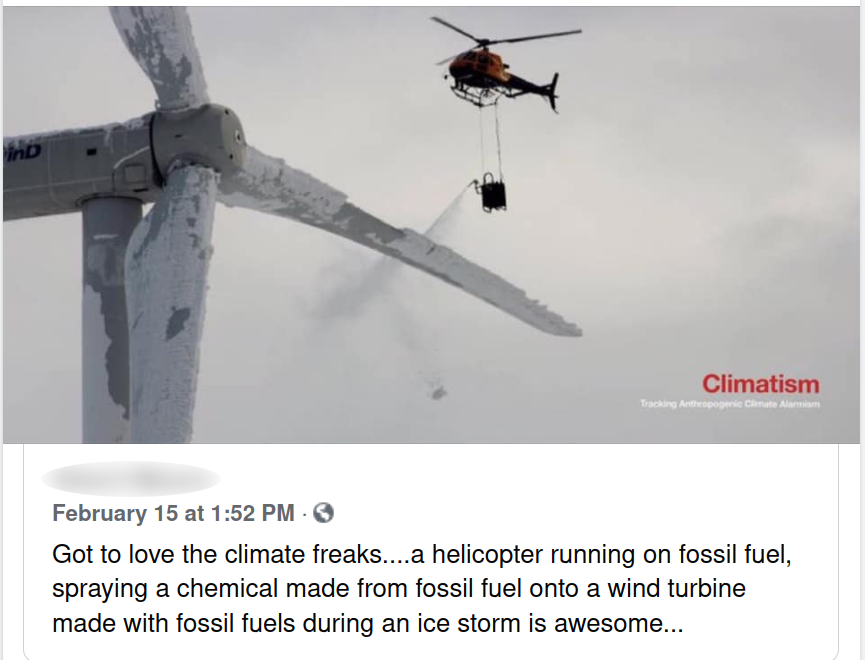
\includegraphics[width=.6\textwidth]{meme.png}
\end{center}



\mynewpage



\begin{question}
  Explain why this meme is bogus. Give links or screenshots to support
  your argument.
  \begin{freeResponse}
    First of all, this is a picture from Sweden, where they use hot
    water to defrost the turbines.
    \begin{center}
      https://apnews.com/article/fact-checking-9953125062
    \end{center}
    Also even if ``hazardous'' de-icing chemicals were used (they
    weren't), the idea that this could offset any benefits from wind
    power, shows a profound misunderstanding of the magnitudes
    involved.  Basically the chemicals and helicopter fuel cannot
    offset energy and environment benefits from wind turbines.
  \end{freeResponse}
\end{question}
\mynewpage

\begin{question}
  After I explained how their meme is bogus, \textit{Geometry Giorgio}
  explains that I was correct, but their ``point'' still stands.

  When I asked \textit{Geometry Giorgio} what their ``point'' was,
  they explain that they are really angry about the Keystone XL
  Pipeline being shut down, because it will cost 1 million
  jobs. \textit{Geometry Giorgio} gives this as evidence:
  \begin{center}
    \texttt{https://mynbc15.com/news/local/berg-pipe-employees-expected-to-lose-job-by-april}
  \end{center}
  What do you think of \textit{Geometry Giorgio}'s claim?  Explain
  your reasoning.
  \begin{freeResponse}
    The article says $106$ people, not $1$ million.
  \end{freeResponse}
\end{question}
\mynewpage


\begin{question}
  After I explained that their claim about jobs was bogus,
  \textit{Geometry Giorgio} then told me that US steel companies would
  be suffering because steel would no longer be needed for the
  pipeline:
  \begin{center}
    \texttt{https://financialpost.com/commodities/energy/keystone-xl-pipeline-tons-scrap-steel}
  \end{center}
  Let's think about this.
  \begin{enumerate}
  \item How many tons of steel are required to finish the Keystone XL
    Pipeline?
  \item What is an approximate weight (in tons) of a wind turbine? 
  \item What percentage of a wind turbine is steel?
  \item How much steel is used in an average wind turbine?
  \item How many wind turbines are installed per year in the United States?
  \item Compare the amount of steel used to complete the Keystone XL
    Pipeline with the amount of steel used to make wind turbines every
    year. What do you say to \textit{Geometry Giorgio}?
  \end{enumerate}
  Give LINKS or SCREENSHOTS to support your numbers in the questions above.
  \begin{freeResponse}
  \item From the article, $660000$ tons of steel are required.
  \item From
    \begin{center}
      https://www.wind-watch.org/publication/nwwpub-size.pdf
    \end{center}
    we see that a typical wind turbine weighs between $164$ and $334$
    tons. So let's assume $249$ tons.
  \item From
    \begin{center}
      https://www.usgs.gov/faqs/what-materials-are-used-make-wind-turbines
    \end{center}
    we see that wind turbines are between $71\%$ and $79\%$ steel, so
    around $75\%$ steel.
  \item So let's estimate that a turbine has
    \[
    0.75\cdot 249 \approx 187~\text{tons of steel}. 
    \]
  \item From
    \[
    https://www.usgs.gov/faqs/how-many-wind-turbines-are-installed-us-each-year
    \]
    we see around $3000$ wind turbines are installed each year.
  \item Now every year, wind turbines account for
    \[
    3000 \cdot 187 = 561000~\text{tons of steel.}
    \]
    This requires almost as much steel as the Keystone Pipeline XL.
    If you are concerned about the steel industry, you should be a fan
    (pun intended) of wind turbines.
  \end{freeResponse}
\end{question}






\end{document}
